% Preamble
\documentclass[11pt,reqno,oneside,a4paper]{article}
\usepackage[a4paper,includeheadfoot,left=25mm,right=25mm,top=00mm,bottom=20mm,headheight=20mm]{geometry}
%%%% DO NOT EDIT THIS FILE

% Standard packages
\usepackage{amssymb,amsmath,amsthm}
\usepackage{xcolor,graphicx}
\usepackage{verbatim}
\usepackage{mathtools}
\usepackage{hyperref}
% Layout of headers & footers
\usepackage{titling}
\usepackage{fancyhdr}
\newcommand{\runningtitle}{Running Title}
\pagestyle{fancy} \lhead{{\theauthor}} \chead{} \rhead{{\runningtitle}} \lfoot{} \cfoot{\thepage} \rfoot{}

% Hyphenation
\hyphenation{non-zero}

% Theorem definitions in the amsthm standard
\newtheorem{thm}{Theorem}
\newtheorem{lem}[thm]{Lemma}
\newtheorem{sublem}[thm]{Sublemma}
\newtheorem{prop}[thm]{Proposition}
\newtheorem{cor}[thm]{Corollary}
\newtheorem{conc}[thm]{Conclusion}
\newtheorem{conj}[thm]{Conjecture}
\theoremstyle{definition}
\newtheorem{defn}[thm]{Definition}
\newtheorem{cond}[thm]{Condition}
\newtheorem{asm}[thm]{Assumption}
\newtheorem{ntn}[thm]{Notation}
\newtheorem{prob}[thm]{Problem}
\theoremstyle{remark}
\newtheorem{rmk}[thm]{Remark}
\newtheorem{eg}[thm]{Example}
\newtheorem*{hint}{Hint}

%% Mathmode shortcuts
% Number sets
\newcommand{\NN}{\mathbb N}              % The set of naturals
\newcommand{\NNzero}{\NN_0}              % The set of naturals including zero
\newcommand{\NNone}{\NN}                 % The set of naturals excluding zero
\newcommand{\ZZ}{\mathbb Z}              % The set of integers
\newcommand{\QQ}{\mathbb Q}              % The set of rationals
\newcommand{\RR}{\mathbb R}              % The set of reals
\newcommand{\CC}{\mathbb C}              % The set of complex numbers
\newcommand{\KK}{\mathbb K}              % An arbitrary field
% Modern typesetting for the real and imaginary parts of a complex number
\renewcommand{\Re}{\operatorname*{Re}} \renewcommand{\Im}{\operatorname*{Im}}
% Upright d for derivatives
\newcommand{\D}{\ensuremath{\,\mathrm{d}}}
% Upright i for imaginary unit
\newcommand{\ri}{\ensuremath{\mathrm{i}}}
% Upright e for exponentials
\newcommand{\re}{\ensuremath{\mathrm{e}}}
% abbreviation for \lambda
\newcommand{\la}{\ensuremath{\lambda}}
% Make epsilons look more different from the element symbol
\renewcommand{\epsilon}{\varepsilon}
% Always use slanted forms of \leq, \geq
\renewcommand{\geq}{\geqslant}
\renewcommand{\leq}{\leqslant}
% Shorthand for "if and only if" symbol
\newcommand{\Iff}{\ensuremath{\Leftrightarrow}}
% Make bold symbols for vectors
\providecommand{\BVec}[1]{\mathbf{#1}}
% Hyperbolic functions
\providecommand{\sech}{\operatorname{sech}}
\providecommand{\csch}{\operatorname{csch}}
\providecommand{\ctnh}{\operatorname{ctnh}}
% sinc function
\providecommand{\sinc}{\operatorname{sinc}}
% closure of a set
\providecommand{\clos}{\operatorname{clos}}
% The absolute value of a real number or modulus of a complex number, with automatically scaling delimiters
\newcommand{\abs}[1]{\left\lvert#1\right\rvert}
\newcommand{\sgn}{\operatorname{sgn}}

% add two sub and superscripts with a space between them
\newcommand{\Mspacer}{\;} %Spacer for below Matrix display functions
\newcommand{\M}[3]{#1_{#2\Mspacer#3}} %Print a symbol with two subscripts eg a matrix entry
\newcommand{\Msup}[4]{#1_{#2\Mspacer#3}^{#4}} %Print a symbol with two subscripts and a superscript eg a matrix entry
\newcommand{\Msups}[5]{#1_{#2\Mspacer#3}^{#4\Mspacer#5}} %Print a symbol with two subscripts and two superscripts eg a matrix entry
\newcommand{\MAll}[7]{\prescript{#1}{#2}{#3}_{#4\Mspacer#5}^{#6\Mspacer#7}} %Print a symbol with two subscripts and two superscripts eg a matrix entry

% Make really wide hat for Fourier transforms applied to large functions
\usepackage{scalerel}
\usepackage{stackengine}
\stackMath
\newcommand\reallywidecheck[1]{%
\savestack{\tmpbox}{\stretchto{%
  \scaleto{%
    \scalerel*[\widthof{\ensuremath{#1}}]{\kern-.6pt\bigwedge\kern-.6pt}%
    {\rule[-\textheight/2]{1ex}{\textheight}}%WIDTH-LIMITED BIG WEDGE
  }{\textheight}%
}{0.5ex}}%
\stackon[1pt]{#1}{\scalebox{-1}{\tmpbox}}%
}
\providecommand{\widecheck}{\reallywidecheck}

\newcommand\reallywidehat[1]{%
\savestack{\tmpbox}{\stretchto{%
  \scaleto{%
    \scalerel*[\widthof{\ensuremath{#1}}]{\kern-.6pt\bigwedge\kern-.6pt}%
    {\rule[-\textheight/2]{1ex}{\textheight}}%WIDTH-LIMITED BIG WEDGE
  }{\textheight}%
}{0.5ex}}%
\stackon[1pt]{#1}{\tmpbox}%
}


%% Acknowledgements
\newcommand{\AckYNCSRP}[1]{#1 gratefully acknowledges support from Yale-NUS College summer research programme.}
\newcommand{\AckYNCProj}[1]{#1 gratefully acknowledges support from Yale-NUS College project B grant IG18-PRB102.}
\newcommand{\AckYNCWorkshop}[1]{#1 gratefully acknowledges support from Yale-NUS College workshop grant IG18-CW003.}
\newcommand{\AckNICA}[1]{#1 would like to thank the Isaac Newton Institute for Mathematical Sciences for support and hospitality during programme \emph{Complex analysis: techniques, applications and computations}, when work on this paper was undertaken. This work was supported by EPSRC Grant Number EP/R014604/1.}
\newcommand{\AckSMRIIVP}[1]{#1 would like to thank the Sydney Mathematics Research Institute for support and hospitality under the International Visitor Programme.}
 % Standard packages, page layout, theorem environments, macros, etc
% This file contains macros specific to the project.
% You are welcome to add your own macros, but please avoid deleting those written by others.

% Asymptotic notation
\newcommand{\bigoh}{\mathcal{O}}
\newcommand{\lindecayla}{\bigoh\left(\abs{\la}^{-1}\right)}
 % Macros specific to this project.
\author{Zhang Liu}
\title{Notes on Complex Analysis}
\renewcommand{\runningtitle}{Notes on Complex Analysis}
\date{\today}

\begin{document}
\maketitle
\thispagestyle{fancy}

\begin{abstract}
    This document is to serve as a set of notes to fill the gaps in my understanding of Complex Analysis relevant to the project. This is thus not intended to be comprehensive, since only the concepts I am currently unfamiliar with will be included. The reference book for this set of notes is \textit{Complex Analysis with Applications} \cite{AG2010a}.
\end{abstract}

% \tableofcontents

\section{The Complex Field} \label{sec:ComplexField}

\begin{defn}
	A complex number $z$ is an ordered pair $(a,b)$ of real numbers. The set of all complex numbers is denoted by $\mathbb{C}$. We think of $\mathbb{C}$ as a vector space over the real numbers, and we define 
	$$1 \equiv (0,0) \text{ and } 0 \equiv (0,1).$$
	Then the set of real numbers $\mathbb{R}$ is contained in $\mathbb{C}$, and for $a,b$ real, we have the identification
	$$(a,b) = a(1,0) + b(0,1) \equiv a1+bi = a + bi.$$
\end{defn}

\par This definition is intuitively very similar to the definition of the vector space over $\mathbb{R}^2$, where $1 \equiv (0,0) \text{ and } 0 \equiv (0,1)$ are analogous to the idea of ``unit vectors," or more generally the basis. This prompted me to explore the similarities and differences between the $\mathbb{R}^2$ and $\mathbb{C}$, through which my initial intuition is proven to be useful only to a limited extent and can be potentially misleading. 

A comparison between $\mathbb{R}^2$ and $\mathbb{C}$:

\begin{enumerate}
	\item The most fundamental distinction is that $\mathbb{R}^2$ is a vector space (over the field of real numbers), whereas $\mathbb{C}$ is a field. 
	
	\item In a vector space of $\mathbb{F}^n$, multiplication between vectors is not defined. 
	
	Recall that we define a vector space to be a set $V$ with an addition and a scalar
	multiplication on $V$. That is, only \textit{scalar} multiplication is defined. In contrast, multiplication is defined on the field of complex numbers, and so are the other algebraic properties associated with multiplication (namely, multiplicative identity, multiplicative inverse, commutativity, associativity of multiplication, and the distributivity law). 
	
	Note that the multiplicative inverse for the field of complex numbers is defined with the concept of the complex conjugate.  
	
	\item A lingering question: is the vector space $\mathbb{C}$ isomorphic to the vector space $\mathbb{R}^2$.

	This question is misleading! A vector space isomorphism is only defined between two vector spaces over the same field. $\mathbb{R}^2$ is a two dimensional field over $\mathbb{R}$ and the vector space $\mathbb{C}$ is a one dimensional vector space over field $\mathbb{C}$.
	 
	However, the field of complex numbers can be viewed as an extension field of $\mathbb{R}$ which treats $\mathbb{C}$ as a two dimensional vector space over R with basis {1, i}. 
	
	The clearest relationship between $\mathbb{C}$ and $\mathbb{R}^2$ is to say that: ``$\mathbb{C}$ is a two dimensional extension field of R."	(See Hungerford’s Algebra, 1974 \cite{Hun1974a}.)
	
	The last point was taken from a set of lecture notes by R. Gardner \cite{Gar2017a}.
\end{enumerate}

\section{Cartesian Form: $z=x +iy$.}

The first way to visualize the complex numbers is to think of them as points in a Cartesian plane. This is achieved by associating each complex number $z=x +iy$ the ordered pair $(x,y)$ and then plot the point $P=(x,y)$ (and hence the construction of the real axis, the imaginary axis, and the complex plane).

Some unfamiliar operations associated with the Cartesian form: 
\begin{itemize}
	\item The Absolute Value (also called the norm or the modulus)
	
	$$\abs{z} = \sqrt{x^2 + y^2},$$
	$$\abs{z_1 - z_2} = \sqrt{(x_1-x_2)^2 + (y_1 - y_2)^2}.$$
	
	\item The Absolute Identity
	$$\abs{z} = \sqrt{z \bar{z}} \text{ or } \abs{z}^2 = z \bar{z},$$
	and its corollaries (refer to AG2010a \cite{AG2010a}). 
	
	\item The Absolute Inequalities
	$$\abs{\Re z} \leq \abs{z}, \abs{\Im z} \leq \abs{z},$$
	$$\abs{z} \leq \abs{\Re z} + \abs{\Im z},$$
	and the triangle inequality: 
	$$\abs{\abs{z_1}-\abs{z_2}} \leq \abs{z_1 + z_2} \leq \abs{z_1} + \abs{z_2},$$
	$$\abs{\abs{z_1}-\abs{z_2}} \leq \abs{z_1 - z_2} \leq \abs{z_1} + \abs{z_2}.$$ 
\end{itemize}

\section{Polar Form: $z = r(\cos\theta + i\sin\theta)$.}
Another useful way to visualize the complex numbers with ``rays from the origin." This is achieved by identifying a complex number with the pair $(r,\theta):$ 
\begin{itemize}
	\item $r$ is the distance from $P$ to the origin $O$, and 
	\item $\theta$ is the angle between the $x$-axis and the ray $OP$. 
\end{itemize}

We define the polar form formally: 

\begin{defn}
	Let $z=x+iy$ be a nonzero complex number. We define a number $r>0$ by setting $r = \sqrt{x^2 + y^2}>0,$ and let $\theta$ be an angle such that 
	
	$$\theta = \frac{x}{\sqrt{x^2 + y^2}} = \frac{x}{r}, \sin \theta = \frac{y}{\sqrt{x^2 + y^2}} = \frac{y}{r}.$$
	
	$r$ is called the modulus of $z$ and $\theta$ the argument of $z$, $z = r(\cos\theta + i\sin\theta).$
\end{defn}

\subsection{Arg z and arg z} An important concept that comes with the polar form is the principle vlaue of the argument, defined as follow:
\begin{defn}
	The \textit{principle value of the argument} of a complex number $z = x+iy$ is the unique number Arg $z$ with the properties: 
	
	\begin{itemize}
		\item $-\pi < \text{Arg }z \leq \pi,$
		\item $\cos(\text{Arg }z) = \frac{x}{\abs{z}},$
		\item $\sin(\text{Arg }z) = \frac{y}{\abs{z}}.$
	\end{itemize}
	With this unique principle value defined, we can then derive the set of all values of argument: $\arg z = \{\text{Arg }z + 2k\pi: k = 0, t_1, t_2,\dots\}.$
	
\end{defn}

\subsection{Arithmetics of the Polar Form}
\begin{itemize}
	\item Multiplication.
	$$z_1 z_2 = r_1 r_2 (\cos(\theta_1 +\theta_2) + i\sin(\theta_1 +\theta_2)).$$
	
	\item Division.
	$$\frac{z_1}{z_2} = \frac{r_1}{r_2} (\cos(\theta+1 - \theta_2) + i\sin(\theta_1-\theta_2)).$$
\end{itemize}

\subsection{Roots of Unity and Solving Equations}

\begin{defn}
	Let $w\neq 0$ be a complex number and $n$ a positive integer. 
	
	A number $z$ is called an $n$th roots of $w$ if $z^n = w$. 
\end{defn}

\begin{prop}
	(De Moivre's Identity) $(\cos \theta +i\sin \theta)^n = \cos n \theta + i\sin n \theta$.
\end{prop}

\begin{rmk}
	Why is de Moivre's formula so significant?
	
	As a result of this work, the credibility of the ``fundamental theorem of algebra” was significantly enhanced, since the objection that Leibniz had raised was definitely answered: it was clear that extraction of roots of complex numbers does not produce imaginary numbers of a new kind. Moreover, since equations of degree at most 4 can be solved by radicals, it follows from de Moivre’s result that polynomials of degree at most 4 split into products of linear factors over the field of complex numbers.  \cite{Tig2016a}.
\end{rmk}

\begin{prop}
	Let $w = \rho (\cos \phi + i\sin \phi) \neq 0.$ The $n$th roots of $w$ are the solutions of the equation $z^n= w$. These are
	$$z_{k+1} = \rho^{\frac{1}{n}}(\cos(\frac{\phi}{n}+\frac{2k\pi}{n})+ i\sin(\theta_1 +\theta_2)),$$
	where $k = 0,1,\dots,n-1$.
\end{prop}

\begin{prop}
	For any positive integer $n$, the $n$ distinct $n$-th roots of $a+bi$ are 
	$$\sqrt[\leftroot{-2}\uproot{2}{2n}]{a^2+b^2}(cos\frac{\varphi+2k\pi}{n} + isin\frac{\varphi+2k\pi}{n})$$
	for $k = 0,\dots,n-1.$
\end{prop}

\begin{rmk}
	From this proposition, it should be observed that, in a rectangular coordinate system, the points $(cos\frac{2k\pi}{n}, sin\frac{2k\pi}{n})$ for $k = 0, 1, . . . , n-1,$ which represent the $n$-th roots unity in the planar representation of $\mathbb{C}$, are the vertices of a regular polygon with $n$ sides: they divide the unit circle into $n$ equal parts. For this reason, the theory which is concerned with n-th roots of unity or with the values of the cosine and sine functions at $2k\pi$ $n$ for integers $k, n$, is called \textbf{\textit{cyclotomy}}, meaning literally ``division of the circle" [into equal parts].
	
	 Likewise, the $n$-th roots of any non-zero complex number are represented in the plane of complex numbers by the vertices of a regular $n$-gon, as the above proposition shows. That the roots of $1$ deserve special interest comes from the fact that, if an $n$-th root $u$ of some complex number $v$ has been found, then the various determinations of $\sqrt[\leftroot{-2}\uproot{2}{n}]{v}$ are the products $\omega u$, where $\omega$ runs over the set of $n$-th roots of unity. This readily follows from 
	$$(\omega u)^n = \omega^nu^n = 1 \cdot un = v$$
	or, equivalently, from the above proposition. \cite{Tig2016a}
\end{rmk}

\begin{defn}
	The unique number $z$ such that 
	$$z^n =w \text{ and Arg }z = \frac{\text{Arg }w}{n},$$
	is called the principal $n$th root of $w$.
	
	The principle root is obtained by taking $\phi = \text{Arg }w$ and $k=0$. 
\end{defn}

A more obvious motivation behind finding the roots of complex numbers is that every complex number has $n$ $n$th roots. A more fundamental motivation for finding the nth roots is to solve polynomial equations of higher degrees. 

While learning on this topic, I have found the discussions on the roots of unity useful in helping develop a better intuition. The following is inspired by the lecture notes by H. Lee \cite{Lee2015a}. 

\begin{defn}
	A complex number $\xi$ is called an $n$-th root of unity, for some integer $n$, if $\xi^n = 1.$
	
	The set of all $n$-th roots of unity is denoted by $\mu_n.$
\end{defn}

The $n$th roots of unity, i.e., roots of 1, satisfy the equation
$$x^n -1 = 0.$$

The $n$th roots of unity, not counting $1$, satisfy
$$\frac{x^n -1 }{x-1} = x^{n-1} + \cdots x+ 1 = 0.$$

The above facts that the sum of the $n$th roots of unity satisfy the equations above, and that their sum is zero can be very useful. Concretely, plugging in the roots of unity can help to factor polynomials and establish divisibility.

This links back to the very reason why complex numbers were first developed: to solve cubic polynomial equations. The usefulness of complex numbers stands out especially in the case where a problem (for example a differential equation) requires us to solve a polynomial equation that may not have real solutions as an intermediate step. Knowing how to work with complex numbers allows us to proceed just as in the real case. 

The above discussion then leads to this final remark that this concept is especailly important in the research on Unifrom Tranform Method because we are ultimately interested in a particular exponential polynomial of higher degree that may require us to solve equations that involve the $n$th roots. 

\section{Complex Functions}

Technically, if we follow the convention for visualizing a real-valued function, then a complex function should be viewed in four-dimensional space. But that is practically impossible and not useful. Thus, we think of a complex function as a mapping from the $z$-plane to the $w$-plane, as shown in the figure below. 

%Reference figures such as figure~\ref{fig:eg} as you need.
% Use this code to insert figures.
\begin{figure}[htp]
	\centering
	% Be sure to save all figures inside the gfx directory or they will NOT be tracked by git
	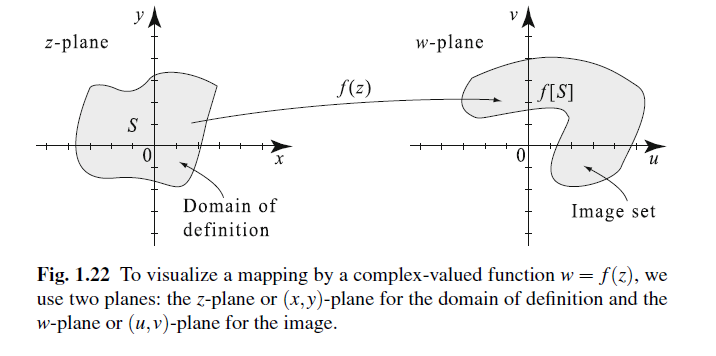
\includegraphics[width=0.8\linewidth]{gfx/complex-function-vis.png}
	\caption{Visualization for A Complex-valued Function}
	\label{fig:complex-function-vis}
\end{figure}
\subsection{Transformations}
\begin{enumerate}
	\item Translations (linear). 
	
	Mappings of the form $z\to z+a+bi$ are \textit{translations} by $a$ units up/down, and $b$ units right/left.
	
	\begin{eg}
		Let $S$ denote the disk $S = \{z:\abs{z} \leq 1\}.$ Find the image of $S$ under the mapping $f(z) = z+2+i$. 
		
		This function translates
		the point z two units to the right and one unit up.
	\end{eg} 
	
	\item Dilations (linear). 
	
	Mappings of the form $z\to rz$, where $r>0$ are \textit{dilations} by a factor $r$. 
	
	\item Rotations (linear).
	
	Mappings of the form $z \to (\cos\theta + i \sin \theta) z$ are \textit{rotations} by the angle $\theta$.
	
	\item Identity (linear). 
	
	Mappings of the form $z\to z$. 
	
	\item Linear Fractional Transformation or Mobius Transformation (non-linear).
	
	Mappings of the form $$z\to w, w = \frac{az+b}{cz+d} (ad\neq bc).$$
	
	\begin{eg}
		A special case: inversion. Inversions are mappings of the form $z \to \frac{1}{z}.$
	\end{eg}
\end{enumerate}

\subsection{Real and Imaginary Parts of Functions}

\par For a complex function $f$, let $u = \Re f$ and $v = \Im f.$ The functions $u,v$ are real-valued functions. With a slight abuse of notation, we can write them as the function for the real part $u(x,y)$ and the function for the imaginary part $v(x,y).$

The motivation behind splitting the complex function into two separate functions, one for the real part and one for the imaginary part is to help us determine algebraically the image of a set when the answer is not geometrically obvious. 

\subsection{Mappings in Polar Coordinates}

Some complex functions and regions are more naturally suited to polar coordinates, especially in our project (and specifically \verb|issue #40|). It is useful to express $w=f(z)$ in polar form: 

$$w=\rho(\cos\phi + i \sin\phi).$$

Using similar logic behind splitting a complex function into $u(x,y)$ and $v(x,y)$, we can identify the polar coordinates of $w$ with a ``modulus function" and an ``argument function," as defined:

$$\rho(r,\theta ) = \abs{f(r\cos\theta + ir\sin\theta)},$$
$$\phi(r,\theta) = \arg (f(r\cos\theta + ir\sin \theta)).$$

\section{The Complex Exponential}

\subsection{Complex Exponential Function: $\exp(z)$ or $e^z$}

\begin{defn}
	We define the \textit{complex exponential function} $\exp(z)$ or $e^z$ as the convergent series:
	$$e^z = \sum_{n=0}^{\infty}\frac{z^n}{n!} = 1 + \frac{z}{1!} + \frac{z^2}{2!} +\cdots, \forall z\in \mathbb{C}.$$
\end{defn}

\begin{rmk}
	This is exactly analogous to the real exponential function:
	$$e^x = 1 + \frac{x}{1!} + \frac{x^2}{2!}+\cdots,$$
	reminding us again of the idea that $\mathbb{C}$ is an extension field of $\mathbb{R}$.
\end{rmk}

Similarly, the properties of the complex exponential function follow exactly as those of the real exponential function. (refer to 1.6.3 to 1.6.5 in AG2010a \cite{AG2010a})

\subsection{Euler's identity and its consequencies}
\begin{prop}
	(Euler's Identity)
	If $z = i\theta,$ where $\theta$ is real, then $$e^{i\theta} = \cos\theta + i\sin\theta.$$
\end{prop}

Using Euler's identity, we can express $e^z$ in terms of the basic functions: $e^x, \cos x, \sin x,$ where $x\in \mathbb{R}$.

\begin{cor}
	For $z=x+iy,$ with $x,y$ real, we have $$e^z = e^x(\cos y + i\sin y) = e^x \cos y + i e^x\sin y.$$
	Taking real and imaginary parts of the above, we find 
	$$\Re(e^z) = e^x \cos y \text{ and } \Im(e^z) = e^x \sin y.$$
\end{cor}

Following from the previous discussion, we also have the facts:
$$\abs{e^z} = e^x >0,$$
$$\arg(e^z) = y + 2k\pi, k \in \mathbb{Z}.$$

Another useful consequence of Euler's Identity is to give rise to an exponential representation of a complex number. To realize that the polar form and exponential form are in fact equivalent, refer to the figure below. 

\begin{prop}
	(Exponential Representation)
	Let $z = r (\cos\theta + i\sin\theta)$ with $r=\abs{z} >0, \theta \in \mathbb{R}, \arg z = \theta + 2k\pi.$ Then 
	$$z = re^{i\theta},$$
	and its corollaries. (see 1.6.17 to 1.6.20 in AG2010a \cite{AG2010a})
\end{prop}

\subsection{The Exponential as a Mapping}

The equation $\arg(e^z) = y + 2k\pi, k \in \mathbb{Z}$ discussed in the previous section has a consequence: the argument of $e^z$ is equal to the imaginary part of $z$. Because of this, we expect the exponential function to map line segments (think the imaginary axis) to circular arcs (think the arc formed due to $\theta$), and by the same logic, rectangular regions to circular regions. 

%Reference figures such as figure~\ref{fig:eg} as you need.
% Use this code to insert figures.
\begin{figure}[htp]
	\centering
	% Be sure to save all figures inside the gfx directory or they will NOT be tracked by git
	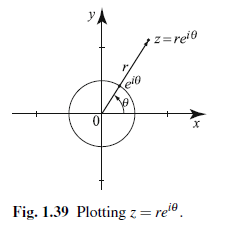
\includegraphics[width=0.4\linewidth]{gfx/exponential-rep.png}
	\caption{Visualization for Exponential Representation}
	\label{fig:exp-rep}
\end{figure}

\section{Relating Trigo Functions to the Exponential Function}

\begin{defn}
	For a complex number $z$, we set
	$$\cos z = \frac{e^{iz} + e^{-iz}}{2},$$
	$$\sin z = \frac{e^{iz} - e^{-iz}}{2i}.$$
\end{defn}
\bibliographystyle{amsplain}
{\small\bibliography{../dbrefs}}
\end{document}
